\documentclass[11pt,a4paper]{article}

\usepackage[utf8]{inputenc}
\usepackage[T1]{fontenc}
\usepackage{lmodern}
\usepackage[margin=1in]{geometry}
\usepackage{amsmath,amssymb,amsthm}
\usepackage{mathtools}
\usepackage{booktabs}
\usepackage{graphicx}
\usepackage{xcolor}
\usepackage{microtype}
\usepackage{listings}
\usepackage{hyperref}

\hypersetup{colorlinks=true, linkcolor=blue!60!black, citecolor=blue!60!black,
            urlcolor=blue!60!black}

\newtheorem{lemma}{Lemma}
\newtheorem{theorem}{Theorem}
\newtheorem{proposition}{Proposition}
\newtheorem{corollary}{Corollary}
\theoremstyle{remark}
\newtheorem{remark}{Remark}

\lstset{basicstyle=\ttfamily\footnotesize, breaklines=true, frame=single,
        columns=fullflexible, keepspaces=true}

% Numbers generated by make_figures.py
% Generated by make_figures.py -- do not edit by hand
\newcommand{\ExpBlo}{23.8}
\newcommand{\ExpBhi}{24.5}
\newcommand{\ExpWidth}{0.7}
\newcommand{\ParS}{49}
\newcommand{\ParSigma}{0.20}
\newcommand{\ParN}{10^{5}}
\newcommand{\ParGap}{0.40}
\newcommand{\ParU}{40{,}000}
\newcommand{\ParA}{20}
\newcommand{\ParLam}{0.036}
\newcommand{\ParGamma}{1.33\times10^{-7}}
\newcommand{\Kone}{0.0489}
\newcommand{\Ktwo}{2.46\times10^{-7}}
\newcommand{\BloPct}{0.100}
\newcommand{\BhiPct}{0.120}
\newcommand{\RelWidth}{0.20}
\newcommand{\Amax}{197}
\newcommand{\Premium}{240{,}053}
\newcommand{\LamStar}{0.036}
\newcommand{\GamSim}{10^{-5}}
\newcommand{\FullFiftyCost}{14.2}
\newcommand{\FullFiftyStd}{29.9}
\newcommand{\FullHundCost}{19.8}
\newcommand{\FullHundStd}{22.1}
\newcommand{\RuleZeroCost}{11.6}
\newcommand{\RuleZeroStd}{26.4}
\newcommand{\RuleHalfCost}{14.1}
\newcommand{\RuleHalfStd}{23.5}
\newcommand{\RuleTwoCost}{19.4}
\newcommand{\RuleTwoStd}{22.1}
\newcommand{\RuleHalfGain}{21}
\newcommand{\ExampleRows}{%
0.050\% & 0.400 & full & 1{,}153 \\
0.105\% & 0.297 & partial & 88 \\
0.112\% & 0.158 & partial & 10 \\
0.130\% & 0.000 & none & 0 \\
}
\newcommand{\ZeroRows}{%
5 & $-$242 & 0.370 \\
20 & $-$130 & 0.189 \\
80 & $-$11 & 0.097 \\
}
\newcommand{\DynRows}{%
Full, 5 dates & -- & 5.0 & 5{,}537 & 89{,}238 \\
Full, 10 dates & -- & 10.0 & 7{,}275 & 64{,}230 \\
Full, 20 dates & -- & 20.0 & 9{,}557 & 45{,}928 \\
Full, 50 dates & -- & 49.9 & 14{,}223 & 29{,}902 \\
Full, 100 dates & -- & 99.6 & 19{,}789 & 22{,}059 \\
\midrule
Rule, 100 dates & $0\,\lambda_*$ & 37.0 & 11{,}561 & 26{,}410 \\
Rule, 100 dates & $0.5\,\lambda_*$ & 46.6 & 14{,}053 & 23{,}526 \\
Rule, 100 dates & $0.9\,\lambda_*$ & 58.4 & 17{,}200 & 22{,}389 \\
Rule, 100 dates & $1.1\,\lambda_*$ & 65.9 & 18{,}517 & 22{,}231 \\
Rule, 100 dates & $2\,\lambda_*$ & 82.0 & 19{,}359 & 22{,}110 \\
}


\newcommand{\E}{\mathbb{E}}
\newcommand{\Var}{\operatorname{Var}}
\newcommand{\NB}{\mathcal{N}}
\newcommand{\F}{\mathcal{F}}
\newcommand{\dd}{\mathrm{d}}

\title{\textbf{Partial rebalancing of a delta hedge under fixed and proportional
transaction costs: a three-phase solution}}
\author{Gagandeep Singh\thanks{M.Sc.\ Physics, TIFR (2024). Independent work.
E-mail: \texttt{gagan45arora@gmail.com}.}}
\date{\today}

\begin{document}
\maketitle

\begin{abstract}
A short option position hedged with the underlying asset carries, between rebalancing
dates, a hedge error: the difference between the model delta and the share holding.
Correcting it incurs a fixed cost per trade and a cost proportional to the traded value.
We determine the cost-optimal size of the correction in a one-period model. To leading
order in the horizon, the P\&L attributable to the hedge error is linear in the error;
any nonlinearity in the value of a correction therefore originates in the risk functional
used to evaluate that P\&L. We prove a general criterion: for a convex risk functional
$\rho$, an interior (partial) correction is optimal only if the proportional cost per unit
traded lies in the interval $(\rho'(0^+), \rho'(u))$, where $u$ is the current hedge
error. A risk functional linear in the P\&L standard deviation gives an empty interval and
hence only full or zero corrections; a functional quadratic in it gives an interval with
lower endpoint zero. For a functional containing both terms, the optimal correction is
obtained in closed form. The parameter space divides into three regions (full, partial,
none) whose boundaries are given explicitly and meet at a triple point. The relative width
of the partial region equals $\gamma uS\sigma\sqrt h/\lambda$, the ratio of the quadratic
to the linear coefficient scaled by the error. We also analyse an earlier exponential risk
functional that produced a partial optimum only for proportional costs near 24\%, and
identify the error in it. A Monte Carlo simulation of the 20-week call example of Hull
compares the rule with full rebalancing on a fixed schedule.
\end{abstract}

\section{Introduction}

Hull's textbook treats the delta hedge of $10^5$ short call options with shares of the
underlying, rebalanced weekly \cite[ch.~19]{hull}. Between rebalancing dates the delta
changes and the share holding is not equal to the model delta. In the absence of
transaction costs the hedge would be restored completely at each date. With a fixed cost
per trade and a proportional cost per unit of traded value, the size of the correction is a
decision variable: given a hedge error of $u$ shares, how many shares $x\in[0,u]$ should
be traded?

This note originated in a numerical calculation. An exponential risk functional, combined
with the two costs, gave an optimum strictly inside $(0,u)$, but only for proportional costs
within about one percentage point of 24\%. Section~\ref{sec:guess} shows that this
functional does not represent the risk of the position. The remaining sections address the
question: \emph{which property of the risk functional determines whether a partial
correction can be optimal?}

Results:
\begin{enumerate}
  \item Lemma~\ref{lem:window}: for convex $\rho$, a partial correction is optimal only if
        the proportional cost per unit traded, $bS$, satisfies
        $\rho'(0^+) < bS < \rho'(u)$.
  \item The hedge-error P\&L is linear in the error (Lemma~\ref{lem:pnl}). A constraint on
        the P\&L standard deviation contributes a term linear in the error; a variance
        penalty contributes a quadratic term (Section~\ref{sec:scores}).
  \item For the combined functional the problem is solved exactly. The parameter space has
        three regions with explicit boundaries and a triple point
        (Theorem~\ref{thm:phases}, Proposition~\ref{prop:boundaries}). The partial region
        has relative width $\gamma uS\sigma\sqrt h/\lambda$ and vanishes as $\gamma\to 0$.
  \item A simulation of the complete 20-week hedge applies the rule at every rebalancing
        date (Section~\ref{sec:sim}).
\end{enumerate}

After this work was completed, the author became aware that no-transaction regions of a
related kind appear in the literature on option hedging with transaction costs, for example
\cite{whalley1997}, where they are derived for a multi-period problem with proportional
costs in the limit of small costs. The present note treats a single decision with fixed and
proportional costs and solves it exactly.

\section{Set-up}\label{sec:setup}

\paragraph{Position.} The position is short $n$ European calls with value $V(t,S)$, long $H$
shares, and a bank account with balance $B$ ($B<0$ denotes borrowing) that accrues interest
at the risk-free rate $r$, $\dd B = rB\,\dd t$. At inception, after the calls are sold and
before any shares are bought, $B = nV_0$. The share price follows
geometric Brownian motion, $\dd S = \mu S\,\dd t + \sigma S\,\dd W$. With delta
$\Delta = \partial V/\partial S$, the share holding that cancels the first-order exposure is
$n\Delta$. The hedge error is
\begin{equation}
  g = n\Delta - H ,
\end{equation}
and in per-option units $g/n = \Delta - \Lambda$, where $\Lambda = H/n\in[0,1]$ is the
hedge ratio. All quantities are real-valued; fractional shares are allowed.

\paragraph{P\&L over a horizon $h$.} The error is assumed to persist for a time $h$, for
example until the next rebalancing date.

\begin{lemma}[Linearity in the hedge error]\label{lem:pnl}
Over $[t,t+h]$ the change in value of $\Pi = -nV + HS + B$ is
\begin{equation}
  \delta\Pi = -g\,\bigl(\delta S - rS h\bigr) + A + o(h),
\end{equation}
where $A$ does not depend on $H$. To leading order in $h$, the term depending on $g$ is
Gaussian with mean $-g(\mu-r)Sh$ and standard deviation $|g|\,S\sigma\sqrt h$.
\end{lemma}

\begin{proof}
By It\^o's formula, $\delta V = \Delta\,\delta S + \tfrac12\Gamma(\delta S)^2 + \Theta h
+ o(h)$. Let $\tilde B = B + HS$ be the balance with the share position converted to
cash; for a given total value of the position, $\tilde B$ does not depend on $H$. The
account accrues $rBh = r\tilde Bh - rHSh$. Then
\[
  \delta\Pi = -(n\Delta - H)\,\delta S - rHSh - n\bigl(\tfrac12\Gamma(\delta S)^2
  + \Theta h\bigr) + r\tilde Bh + o(h).
\]
Adding and subtracting $rn\Delta Sh$ gives the stated form with
$A = -n(\tfrac12\Gamma(\delta S)^2 + \Theta h) + r\tilde Bh - rn\Delta Sh$, independent of $H$.
With $\delta S = S(\mu h + \sigma\sqrt h\,Z)$, $Z\sim\mathcal N(0,1)$, the $g$-term has the
stated mean and standard deviation. Its covariance with $A$ involves
$\E[(\delta S - \E\delta S)^3] = O(h^2)$ and $\E[\delta S]\Var[\delta S] = O(h^2)$, both
$o(h)$.
\end{proof}

The $g$-dependent part of $\delta\Pi$ is linear in $g$. The position therefore supplies no
curvature in $g$; any dependence of the marginal value of a correction on the size of the
remaining error must come from the risk functional applied to $\delta\Pi$.

The drift term $-g(\mu-r)Sh$ is a directional exposure and is excluded from the hedging
objective, which is equivalent to setting $\mu = r$ in the evaluation of the error.
Retaining it shifts the target holding by a constant and does not change the structure of
the results.

\paragraph{Decision problem.} Let $u = |g| > 0$ and, without loss of generality, $g>0$.
Buying $x\in[0,u]$ shares reduces the error to $u-x$. Trades with $x>u$ or in the opposite
direction are dominated: for $x>u$, the trade $2u-x$ leaves an error of equal magnitude at
lower cost. A trade of $x>0$ shares costs
\begin{equation}
  c(x) = a + bSx , \qquad c(0) = 0,
\end{equation}
with fixed cost $a\ge 0$ and proportional cost $b\ge 0$. Let $\rho(g)\ge 0$, $\rho(0)=0$, be
the risk functional, in dollars, assigned to an error $g$ held over the horizon. The net
benefit of trading $x$ shares is
\begin{equation}
  \NB(x) = \rho(u) - \rho(u - x) - c(x), \qquad \NB(0) = 0,
  \label{eq:net}
\end{equation}
and the problem is $x^* = \arg\max_{x\in[0,u]}\NB(x)$.

\section{A necessary condition for partial correction}\label{sec:lemma}

Let $\beta = bS$ denote the marginal transaction cost per share. On $(0,u]$,
\begin{equation}
  \NB'(x) = \rho'(u - x) - \beta .
\end{equation}
The argument of $\rho'$ is the \emph{remaining} error $u - x$. At the start of the trade
($x\to 0^+$) the remaining error is $u$; at the end ($x = u$) it is $0$. The slope of $\NB$
at the two ends is therefore
\begin{equation}
  \NB'(0^+) = \rho'(u) - \beta, \qquad \NB'(u) = \rho'(0^+) - \beta .
  \label{eq:endslopes}
\end{equation}
If $\rho$ is convex, $\rho'(u-x)$ is non-increasing in $x$, so $\NB'$ decreases from
$\NB'(0^+)$ to $\NB'(u)$. Since $c$ jumps by $a$ at $x=0$, $\lim_{x\to0^+}\NB(x) = -a$.

\begin{lemma}[Marginal-cost interval]\label{lem:window}
Let $\rho$ be convex on $[0,u]$ and differentiable on $(0,u]$, with right derivative
$\rho'(0^+)$ at $0$.
\begin{enumerate}
  \item If $\NB'(u)\ge 0$, i.e.\ $\beta\le\rho'(0^+)$: $\NB$ is non-decreasing on
        $(0,u]$. The candidates are $x=u$ and $x=0$; $x^*=u$ (\emph{full}) if
        $\NB(u)>0$, otherwise $x^*=0$.
  \item If $\NB'(0^+)>0>\NB'(u)$, i.e.\ $\rho'(0^+)<\beta<\rho'(u)$: $\NB$ increases and
        then decreases on $(0,u]$. The candidates are $\hat x\in(0,u)$ with
        $\NB'(\hat x)=0$, i.e.\ $\rho'(u-\hat x)=\beta$ (unique if $\rho$ is strictly
        convex), and $x=0$; $x^*=\hat x$ (\emph{partial}) if $\NB(\hat x)>0$, otherwise
        $x^*=0$.
  \item If $\NB'(0^+)\le 0$, i.e.\ $\beta\ge\rho'(u)$: $\NB$ is non-increasing on $(0,u]$
        and bounded above by $-a\le 0$, so $x^*=0$ (\emph{none}).
\end{enumerate}
\end{lemma}

\begin{proof}
Case 1: $\NB'(x)\ge\NB'(u)\ge 0$ on $(0,u]$, so $\max_{(0,u]}\NB = \NB(u)$. Case 3:
$\NB'(x)\le\NB'(0^+)\le 0$ on $(0,u]$, so $\sup_{(0,u]}\NB = \lim_{x\to0^+}\NB = -a \le 0
= \NB(0)$. Case 2: $\NB'$ is non-increasing, positive near $0$ and negative near $u$, so
$\max_{(0,u]}\NB$ is attained where $\NB'$ changes sign. In each case the maximum over
$(0,u]$ is compared with $\NB(0)=0$.
\end{proof}

Figure~\ref{fig:cases} shows the three cases for the risk functional of
Section~\ref{sec:scores}. In terms of marginal quantities: $\rho'(u)$ is the marginal risk
reduction per share at the start of the trade, $\rho'(0^+)$ the marginal risk reduction as
the error reaches zero, and $\beta$ the marginal cost. An interior optimum exists only if the
marginal cost lies strictly between these two values. The length of this interval is
\begin{equation}
  \rho'(u) - \rho'(0^+) = \int_0^u \rho''(g)\,\dd g .
  \label{eq:width}
\end{equation}
\begin{figure}[htbp]
  \centering
  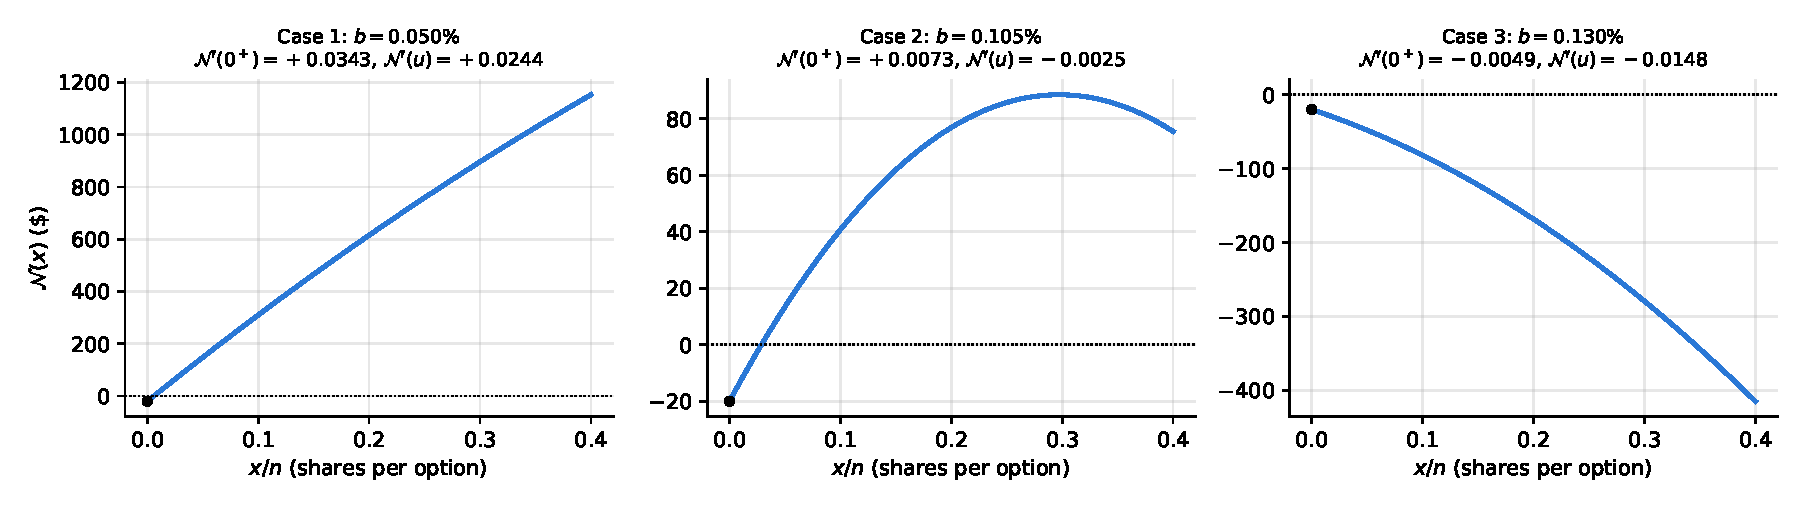
\includegraphics[width=\textwidth]{figures/fig_cases.pdf}
  \caption{Net benefit $\NB(x)$ in the three cases of Lemma~\ref{lem:window}, for the
  functional and parameters of Sections~\ref{sec:scores} and~\ref{sec:numbers}. The dot
  marks $\lim_{x\to0^+}\NB = -a$; the titles give the end slopes \eqref{eq:endslopes}.}
  \label{fig:cases}
\end{figure}

Two consequences:
\begin{itemize}
  \item if $\rho$ is linear in $|g|$, the interval is empty and $x^*\in\{0,u\}$;
  \item if $\rho'(0^+) = 0$, the interval is $(0,\rho'(u))$, so for every
        $0 < b < \rho'(u)/S$ any trade made is partial and $x^* = u$ never occurs.
\end{itemize}

\section{An exponential risk functional}\label{sec:guess}

The calculation that motivated this note used
\begin{equation}
  \rho_{\rm exp}(g) = S\exp\!\Bigl(g\mu\tau - \tfrac12 g^2\sigma^2\tau + g\sigma\sqrt\tau\Bigr),
\end{equation}
with $\tau$ the time to expiry, $g$ in shares per option, and transaction costs compounded to
expiry by $e^{r\tau}$. For $S = 49$, $\sigma = 0.2$, $\mu = r = 0.05$, $\tau = 1$, $u = 0.4$
per option and $a = 0.02$, $\rho_{\rm exp}$ is convex on $[0,u]$ and Lemma~\ref{lem:window}
gives the interval
\[
  \ExpBlo\% < b < \ExpBhi\% ,
\]
of length $\ExpWidth$ percentage points, at $b$ of order $\sigma\sqrt\tau = 20\%$
(Figure~\ref{fig:guess}). For all smaller $b$ the optimum is $x^* = u$.

\begin{figure}[htbp]
  \centering
  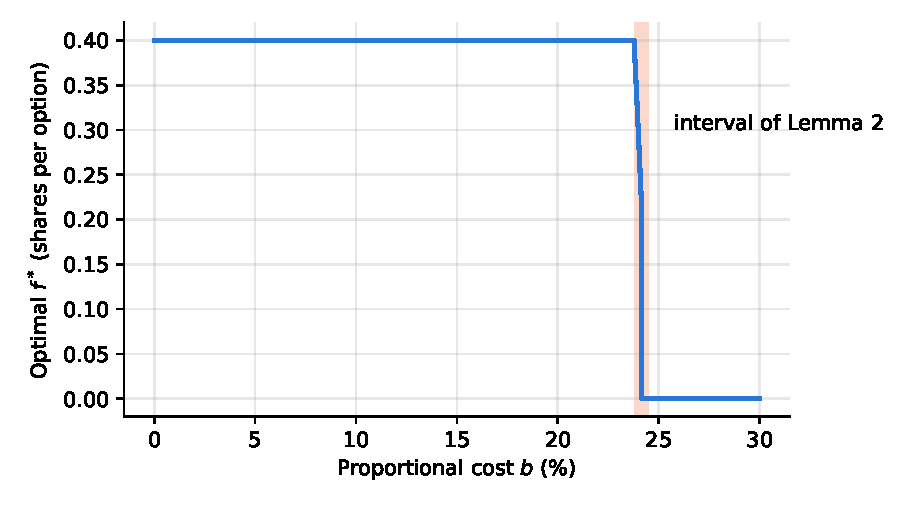
\includegraphics[width=0.66\textwidth]{figures/fig_first_guess.pdf}
  \caption{Exponential risk functional: optimal correction as a function of the
  proportional cost $b$. The shaded interval is that of Lemma~\ref{lem:window}.}
  \label{fig:guess}
\end{figure}

The functional is not a risk measure of the hedge error:
\begin{itemize}
  \item It has the form of the $+1\sigma$ terminal value of a portfolio continuously
        rebalanced to hold a constant fraction $g$ of its wealth in the stock, for which
        $\log(\text{wealth}/\text{initial}) = (r + g(\mu - r))\tau - \tfrac12g^2\sigma^2\tau
        + g\sigma W_\tau$. The hedge error is a static share position whose P\&L is linear
        in $g$ (Lemma~\ref{lem:pnl}); the curvature of $\rho_{\rm exp}$ in $g$ belongs to
        the constant-fraction portfolio, not to the hedge error.
  \item $g$ is a number of shares per option but enters as a wealth fraction, and the
        prefactor $S$ is a share price, not a wealth.
  \item $\rho_{\rm exp}(0) = S \ne 0$, so a zero error is assigned nonzero risk.
\end{itemize}
The one-standard-deviation loss of the hedge error, $|g|\,S\sigma\sqrt h$
(Lemma~\ref{lem:pnl}), is linear in $|g|$; by Lemma~\ref{lem:window} its interval is empty.
The interval in Figure~\ref{fig:guess} is therefore a consequence of the incorrect
functional. Curvature in $g$ has to be introduced through the risk functional.

\section{Risk functionals for the hedge error}\label{sec:scores}

Let $X$ be the hedge-error P\&L over the horizon. By Lemma~\ref{lem:pnl}, with the drift
excluded, $X$ is Gaussian with mean zero and standard deviation $s(g) = |g|\,S\sigma\sqrt h$.

\paragraph{(a) Variance penalty.} Evaluate a random P\&L $X$ by
\begin{equation}
  \F_\gamma[X] = -\frac1\gamma\log\E\bigl[e^{-\gamma X}\bigr], \qquad \gamma > 0 ,
\end{equation}
the free energy of $X$ at inverse temperature $\gamma$ (units 1/\$). Negative outcomes are
weighted by $e^{-\gamma X}$; $\F_\gamma\to\E X$ as $\gamma\to 0$. The cumulant expansion is
\begin{equation}
  \F_\gamma[X] = \kappa_1 - \tfrac{\gamma}{2}\kappa_2 + \tfrac{\gamma^2}{6}\kappa_3 - \dots ,
\end{equation}
which terminates at $\E X - \tfrac{\gamma}{2}\Var X$ for Gaussian $X$. The hedge error
therefore contributes
\begin{equation}
  \rho_{\rm var}(g) = \tfrac12\gamma S^2\sigma^2h\,g^2 .
\end{equation}

\paragraph{(b) Constraint on the standard deviation.} Impose $s(g)\le L_{\max}$ on the
position. Maximising $\F_\gamma$ under this constraint with Lagrange multiplier
$\lambda\ge 0$ is equivalent to maximising $\F_\gamma - \lambda\,(s - L_{\max})$. By
complementary slackness $\lambda = 0$ if the constraint is inactive and $\lambda>0$ if it is
active; $\lambda$ is dimensionless (dollars of objective per dollar of standard deviation).
The hedge error contributes
\begin{equation}
  \rho_{\rm sd}(g) = \lambda S\sigma\sqrt h\,|g| ,
\end{equation}
which is linear in $|g|$ because the standard deviation is homogeneous of degree one in the
position. Hull describes trading desks operating under limits on the Greeks of their
positions \cite[ch.~19]{hull}; a constraint on $s$ is of the same type.

\paragraph{Combined functional.}
\begin{equation}
  \boxed{\;\rho(g) = k_1|g| + \tfrac12k_2g^2, \qquad
  k_1 = \lambda S\sigma\sqrt h, \quad k_2 = \gamma S^2\sigma^2 h\;}
  \label{eq:rho}
\end{equation}
with $k_1$ in \$/share and $k_2$ in \$/share$^2$. Both coefficients are built from the
one-share standard deviation $S\sigma\sqrt h$, to the first and second power respectively.
In Lemma~\ref{lem:window}, $\rho'(0^+) = k_1$ and $\rho'' = k_2$, so the interval is
$(k_1,\,k_1 + k_2u)$ with length $k_2u$. The linear term makes $x^* = u$ attainable for
$b>0$; the quadratic term gives the interval nonzero length.

\section{Solution}\label{sec:solution}

With \eqref{eq:rho},
\begin{equation}
  \rho(u) - \rho(u-x) = (k_1 + k_2u)\,x - \tfrac12 k_2x^2 ,
\end{equation}
which is concave in $x$, and for $x>0$
\begin{equation}
  \NB(x) = (k_1 + k_2u - bS)\,x - \tfrac12k_2x^2 - a .
\end{equation}
Define
\begin{equation}
  w = \frac{bS - k_1}{k_2}.
\end{equation}

\begin{theorem}[Optimal correction]\label{thm:phases}
Let $k_1\ge 0$, $k_2>0$. Then
\begin{equation}
  x^* =
  \begin{cases}
    u     & \text{(full)} \quad\ \ \text{if } bS\le k_1 \text{ and }
            (k_1 - bS)\,u + \tfrac12k_2u^2 > a,\\[2pt]
    u - w & \text{(partial)} \ \text{if } k_1 < bS < k_1 + k_2u \text{ and }
            \tfrac12k_2(u-w)^2 > a,\\[2pt]
    0     & \text{(none)} \quad\ \text{otherwise.}
  \end{cases}
  \label{eq:xstar}
\end{equation}
In the partial region $\NB(x^*) = \tfrac12k_2(u-w)^2 - a$, and the residual error is $w$,
independent of $u$.
\end{theorem}

\begin{proof}
$\rho$ is convex on $[0,u]$ with $\rho'(g) = k_1 + k_2g$ on $(0,u]$ and $\rho'(0^+) = k_1$;
apply Lemma~\ref{lem:window} with interval $(k_1,\,k_1+k_2u)$.
\emph{Full:} $\NB(u) = (k_1 - bS)u + \tfrac12k_2u^2 - a$.
\emph{Partial:} $\rho'(u-\hat x) = bS$ gives $u - \hat x = w$, with $0<w<u$ inside the
interval. Since $k_1 + k_2u - bS = k_2(u - w)$,
\[
  \NB(\hat x) = k_2(u-w)^2 - \tfrac12k_2(u-w)^2 - a = \tfrac12k_2(u-w)^2 - a .
\]
\emph{None:} case 3 of the lemma, or $\NB\le 0$ at the candidate.
\end{proof}

The fixed cost $a$ enters only the conditions $\NB>0$; it does not affect the value of
$x^*$ in the partial region. The residual error after a partial correction is $w$
regardless of the initial error $u$.

\begin{proposition}[Region boundaries]\label{prop:boundaries}
For fixed $u$, the boundaries in the $(b,a)$ plane are
\begin{align}
  \text{full | partial:} &\quad b = b_0 \equiv \frac{k_1}{S}, && 0\le a\le a_c,
    \label{eq:fp}\\
  \text{partial | none:} &\quad b = \frac{k_1 + k_2u - \sqrt{2k_2a}}{S}, && 0\le a\le a_c,
    \label{eq:pn}\\
  \text{full | none:}    &\quad b = \frac{k_1 + \tfrac12k_2u - a/u}{S}, && a\ge a_c,
    \label{eq:fn}
\end{align}
with $a_c = \tfrac12k_2u^2$. The three curves meet at the triple point $(b_0, a_c)$. The
partial region is non-empty only for $a < a_c$; at $a = 0$ it is
$b\in(b_0,\, b_0 + k_2u/S)$.
\end{proposition}

\begin{proof}
\eqref{eq:fp} is the boundary $bS = k_1$ of case 1. On it the full and partial candidates
coincide ($w = 0$) with $\NB = \tfrac12k_2u^2 - a$, so it separates the full and partial
regions if and only if $a < a_c$. \eqref{eq:pn} is the solution of $\tfrac12k_2(u-w)^2 = a$
for $b$, and \eqref{eq:fn} the solution of $(k_1 - bS)u + \tfrac12k_2u^2 = a$. At $a = a_c$
both give $b = b_0$.
\end{proof}

\begin{corollary}[Width of the partial region; limits]\label{cor:width}
At $a=0$ the relative width of the partial region is
\begin{equation}
  \frac{k_2u}{k_1} = \frac{\gamma\,(uS\sigma\sqrt h)}{\lambda} ,
\end{equation}
a dimensionless ratio: $\gamma$ times the standard deviation of the P\&L of the full error,
divided by $\lambda$. In the limits:
\begin{itemize}
  \item $\gamma\to 0$: the partial region contracts to the line $b = b_0$ and
        $x^*\in\{0,u\}$;
  \item $\lambda\to 0$: $b_0\to 0$, the full region is empty for $b>0$, and every nonzero
        $x^*$ is partial.
\end{itemize}
The partial region is narrow compared with $b_0$ if and only if
$\gamma\,uS\sigma\sqrt h \ll \lambda$.
\end{corollary}

\begin{remark}[Dependence on $h$]\label{rem:h}
Since $k_1\propto\sqrt h$ and $k_2\propto h$, the relative width scales as $\sqrt h$. The
boundary $b_0 = \lambda\sigma\sqrt h$ is independent of $S$.
\end{remark}

\section{Numerical example}\label{sec:numbers}

Parameters: $S = \ParS$, $\sigma = \ParSigma$, $n = \ParN$ options, error $\ParGap$ shares
per option ($u = \ParU$ shares), $h = 1/52$ year, $a = \$\ParA$, $\lambda = \ParLam$,
$\gamma = \ParGamma$ per dollar. The values of $\lambda$ and $\gamma$ are illustrative and
are not calibrated. They give
\begin{gather*}
  k_1 = \Kone\ \$/\text{share},\qquad k_2 = \Ktwo\ \$/\text{share}^2,\\
  b_0 = \BloPct\%,\qquad b_0 + k_2u/S = \BhiPct\%,\qquad
  \frac{k_2u}{k_1} = \RelWidth,\qquad a_c = \$\Amax .
\end{gather*}

\begin{table}[htbp]
\centering
\caption{Optimal correction at four values of the proportional cost.}
\label{tab:examples}
\begin{tabular}{rrlr}
\toprule
$b$ & $f^* = x^*/n$ & Region & $\NB(x^*)$ (\$) \\
\midrule
\ExampleRows
\bottomrule
\end{tabular}
\end{table}

Figure~\ref{fig:hills} shows $\NB(f)$ for the four values of Table~\ref{tab:examples}.
Figure~\ref{fig:fstar} shows $f^*(b)$: $f^* = u/n$ for $b\le b_0$, a decreasing segment in
the partial region, and $f^*=0$ beyond it. The length of the decreasing segment grows with
$\gamma$, consistent with Corollary~\ref{cor:width}. Figure~\ref{fig:phase} shows the
regions in the $(b,a)$ plane, evaluated pointwise from \eqref{eq:xstar}, with the boundaries
\eqref{eq:fp}--\eqref{eq:fn} superimposed. A grid maximisation of $\NB$ reproduces the
closed-form $x^*$ at all values tested.

\begin{figure}[htbp]
  \centering
  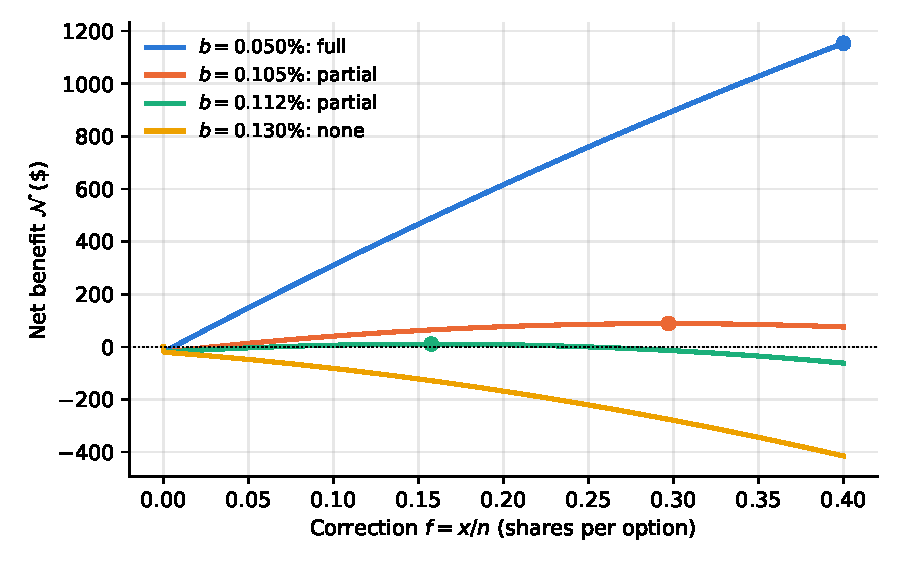
\includegraphics[width=0.68\textwidth]{figures/fig_hills.pdf}
  \caption{Net benefit $\NB$ against the correction per option, for the values of $b$ in
  Table~\ref{tab:examples}. Markers indicate $x^*$ where $x^*>0$.}
  \label{fig:hills}
\end{figure}

\begin{figure}[htbp]
  \centering
  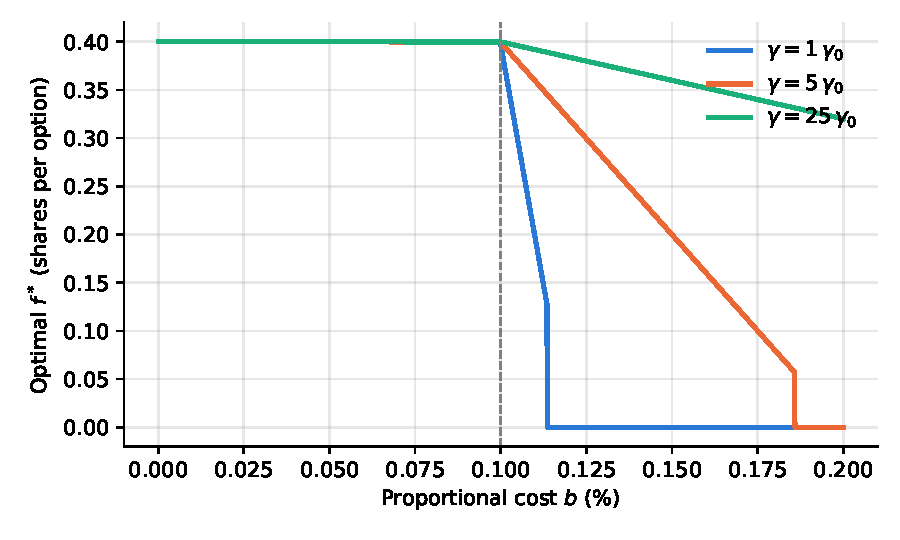
\includegraphics[width=0.68\textwidth]{figures/fig_fstar.pdf}
  \caption{Optimal correction per option against $b$ for three values of $\gamma$
  ($\gamma_0 = \ParGamma$). Dashed line: $b = b_0$.}
  \label{fig:fstar}
\end{figure}

\begin{figure}[htbp]
  \centering
  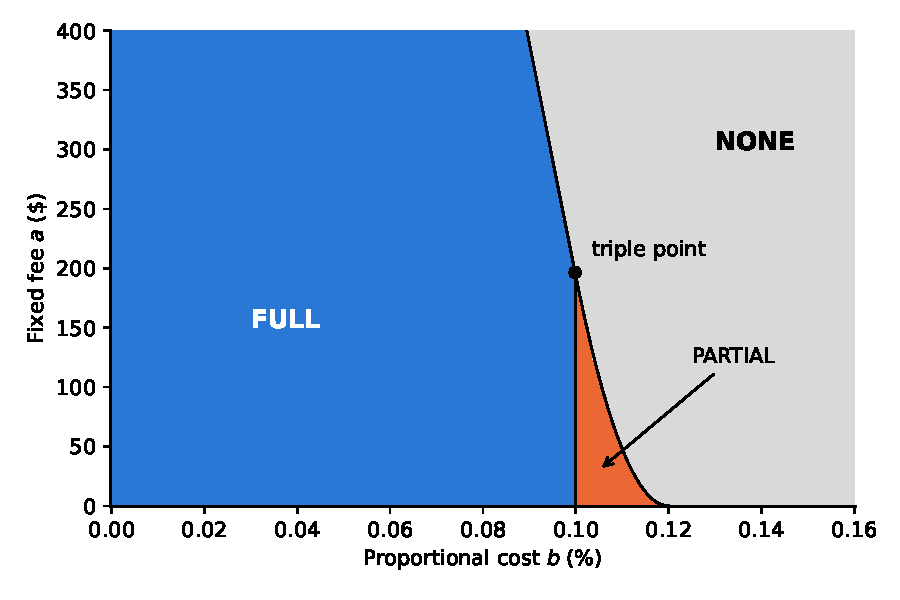
\includegraphics[width=0.68\textwidth]{figures/fig_phase.pdf}
  \caption{Regions in the $(b,a)$ plane: full (blue), partial (orange), none (grey). Black
  curves: boundaries \eqref{eq:fp}--\eqref{eq:fn}, meeting at the triple point
  $(b_0, a_c)$.}
  \label{fig:phase}
\end{figure}

\section{Simulation of the complete hedge}\label{sec:sim}

Theorem~\ref{thm:phases} concerns a single decision. To examine repeated application, we
simulate the example of \cite[ch.~19]{hull}: $10^5$ short calls with $S_0 = 49$, $K = 50$,
$r = 0.05$, $\sigma = 0.2$ and 20 weeks to expiry, sold at the Black--Scholes price
(\$$\Premium$ in total). The share price follows geometric Brownian motion with
$\mu = 0.13$. The bank account accrues at $r$ and is charged for share purchases and
transaction costs. At expiry the shares are valued at $S_T$ and the payoff is paid. Transaction costs are $a = \$20$ and $b = 0.1\%$. Each strategy is evaluated on
the same $10^4$ paths.

Without transaction costs and with full rebalancing at $m$ equally spaced dates, the mean
P\&L is consistent with zero and its standard deviation divided by the premium decreases
approximately as $m^{-1/2}$ (Table~\ref{tab:zero}), consistent with Hull's results.

\begin{table}[htbp]
\centering
\caption{No transaction costs; full rebalancing at $m$ dates.}
\label{tab:zero}
\begin{tabular}{rrr}
\toprule
$m$ & Mean P\&L (\$) & Std.\ dev.\ / premium \\
\midrule
\ZeroRows
\bottomrule
\end{tabular}
\end{table}

With transaction costs two strategy families are compared:
\begin{itemize}
  \item full rebalancing at $m\in\{5,10,20,50,100\}$ equally spaced dates;
  \item rule \eqref{eq:xstar} evaluated at 100 equally spaced dates, with $h = 1/52$,
        $\gamma = \GamSim$ per dollar and $\lambda$ a multiple of
        $\lambda_* = b/(\sigma\sqrt h) = \LamStar$, the value for which $b = b_0$.
\end{itemize}
By Theorem~\ref{thm:phases}, for $\lambda<\lambda_*$ every nonzero trade is partial; for
$\lambda>\lambda_*$ every nonzero trade is full.

\begin{table}[htbp]
\centering
\caption{Complete hedge: mean number of trades per path, mean transaction cost, and
standard deviation of the final P\&L (present values, \$).}
\label{tab:dyn}
\begin{tabular}{lcrrr}
\toprule
Strategy & $\lambda$ & Trades & Mean cost & Std.\ dev. \\
\midrule
\DynRows
\bottomrule
\end{tabular}
\end{table}

\begin{figure}[htbp]
  \centering
  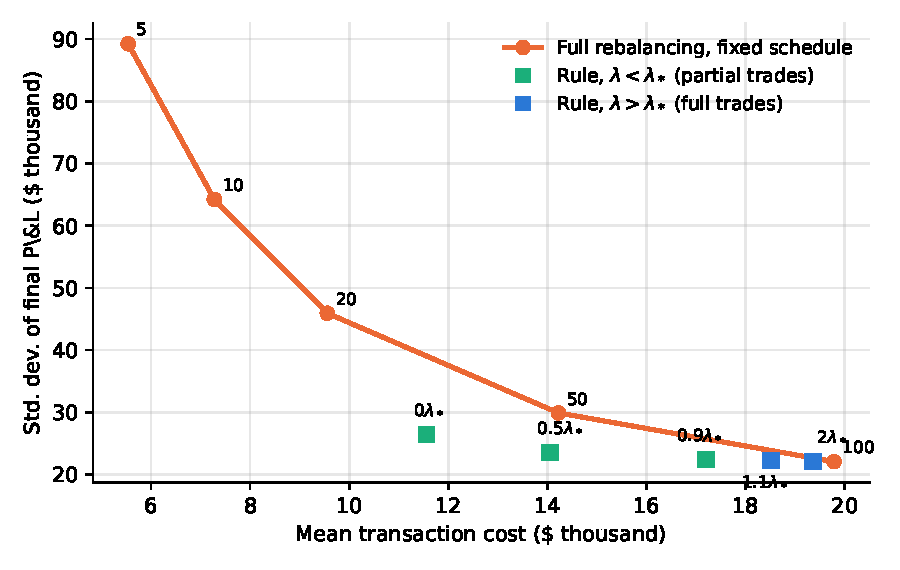
\includegraphics[width=0.68\textwidth]{figures/fig_dynamic.pdf}
  \caption{Mean transaction cost against standard deviation of the final P\&L. Labels on
  the full-rebalancing curve give $m$.}
  \label{fig:dyn}
\end{figure}

Results (Table~\ref{tab:dyn}, Figure~\ref{fig:dyn}):
\begin{itemize}
  \item $\lambda = 0.5\lambda_*$: mean cost \$$\RuleHalfCost$k and standard deviation
        \$$\RuleHalfStd$k, against \$$\FullFiftyCost$k and \$$\FullFiftyStd$k for full
        rebalancing at 50 dates: equal cost to within 2\%, $\RuleHalfGain\%$ lower
        standard deviation.
  \item $\lambda = 0$: \$$\RuleZeroCost$k and \$$\RuleZeroStd$k, lower in both quantities
        than full rebalancing at 50 dates.
  \item $\lambda = 2\lambda_*$: \$$\RuleTwoCost$k and \$$\RuleTwoStd$k, within 3\% in cost
        and 1\% in standard deviation of full rebalancing at 100 dates
        (\$$\FullHundCost$k, \$$\FullHundStd$k). In this case all trades are full and the
        rule differs from the 100-date schedule only by omitting trades for small errors.
\end{itemize}
The configurations with partial trades ($\lambda<\lambda_*$) lie below the full-rebalancing
curve in Figure~\ref{fig:dyn}; those with full trades ($\lambda>\lambda_*$) lie close to its
100-date end point.

\section{Limitations}\label{sec:limits}

\begin{itemize}
  \item \textbf{Single period.} The functional evaluates the error over one horizon $h$ and
        omits the cost of later corrections of the residual error. The results depend on
        $h$ (Remark~\ref{rem:h}). The multi-period problem is a dynamic-programming problem
        and is not treated here.
  \item \textbf{Constant error over the horizon.} Changes in $\Delta$ during the horizon
        (gamma) are neglected at leading order.
  \item \textbf{Gaussian approximation.} $\F_\gamma = \E X - \tfrac\gamma2\Var X$ holds
        exactly only for Gaussian $X$; non-zero third and higher cumulants of an option
        position contribute at higher order in $\gamma$.
  \item \textbf{Parameters.} $\lambda$ and $\gamma$ are illustrative. A calibration, for
        example to a target standard deviation of the final P\&L, is not performed.
  \item \textbf{Cost model.} Market impact, size-dependent proportional costs and the cost
        of closing the position at expiry are not included.
\end{itemize}

\section{Summary}

To leading order in the horizon, the P\&L of a delta-hedge error is linear in the error, so
the dependence of the optimal correction on the error size is determined by the risk
functional. For convex $\rho$, a partial correction is optimal only if $bS$ lies in
$(\rho'(0^+), \rho'(u))$ (Lemma~\ref{lem:window}). A functional linear in the P\&L standard
deviation gives an empty interval; a variance penalty gives an interval with lower endpoint
zero. For the combined functional $\rho = k_1|g| + \tfrac12k_2g^2$ the optimal correction
is given in closed form, with three regions in the $(b,a)$ plane, explicit boundaries and a
triple point at $(k_1/S,\,\tfrac12k_2u^2)$. The partial region has relative width
$\gamma uS\sigma\sqrt h/\lambda$. An exponential functional that produced partial optima
only near $b = 24\%$ was shown not to represent the risk of the hedge error. In the
simulated 20-week hedge, configurations of the rule with partial trades attain lower
P\&L standard deviation than full rebalancing on a fixed schedule at equal mean cost.

\appendix
\section{Implementation}

All figures and tables are produced by \texttt{make\_figures.py}. Implementation of
\eqref{eq:xstar}:

\begin{lstlisting}[language=Python]
def decide(u, S, b, a, k1, k2):
    """Optimal number of shares to trade for a hedge error u >= 0 (Theorem 1)."""
    c = b * S                              # marginal cost per share
    if c <= k1:                            # marginal cost <= rho'(0+): full candidate
        x = u
    elif k2 > 0 and c < k1 + k2 * u:       # rho'(0+) < c < rho'(u): interior candidate
        x = u - (c - k1) / k2
    else:                                  # c >= rho'(u): no trade
        return 0.0
    gain = (k1 + k2 * u) * x - 0.5 * k2 * x**2 - (a + c * x)
    return x if gain > 0 else 0.0
\end{lstlisting}

\begin{thebibliography}{9}
\bibitem{hull}
J.~C. Hull, \emph{Options, Futures, and Other Derivatives}, 11th ed., Pearson, 2021.

\bibitem{whalley1997}
A.~E. Whalley and P.~Wilmott, An asymptotic analysis of an optimal hedging model for option
pricing with transaction costs, \emph{Mathematical Finance} \textbf{7}(3), 307--324, 1997.
\end{thebibliography}

\end{document}
